% 01-metodologija.tex - METODOLOGIJA

\section{TEORIJSKE OSNOVE I UPRAVLJAČKE STRATEGIJE}
\label{sec:metodologija}

Uspješno autonomno robotsko ultrazvučno snimanje zahtijeva pažljivo odabranu strategiju upravljanja interakcijom između robota i mekog tkiva pacijenta. Tradicionalne metode upravljanja industrijskim robotima primarno su usmjerene na praćenje unaprijed definiranih geometrijskih putanja u prostoru bez obzira na sile koje se pri tome javljaju. U medicinskom okruženju takav je pristup neprikladan i potencijalno vrlo opasan.

\subsection{Pozicijsko upravljanje i njegova ograničenja}
Pozicijsko upravljanje (engl. \textit{position control}) nastoji minimalizirati pogrešku položaja krajnjeg efektora robota u odnosu na zadanu putanju $x_d(t)$. Upravljački algoritam generira upravljačke momente u zglobovima kako bi nadvladao sve vanjske sile i održao zadanu poziciju. 
U robotskoj ehografiji pozicijsko upravljanje pati od sljedećih kritičnih nedostataka \cite{qin2026review, mathworks2025advanced}:
\begin{itemize}
    \item \textbf{Sigurnosni rizik:} Ako se pacijent pomakne prema robotu ili ako je geometrijski model tijela netočan, pozicijski kontroler će pokušati dosegnuti zadanu točku unutar tijela, što dovodi do nekontroliranog rasta kontaktne sile i opasnosti od ozljeda.
    \item \textbf{Gubitak akustičkog kontakta:} Ako je stvarna površina tijela niža od modelirane, sonda će lebdjeti iznad kože, što onemogućuje prijenos ultrazvučnih valova.
    \item \textbf{Osjetljivost na deformacije tkiva:} Zbog elastičnosti kože i potkožnog tkiva, fiksna pozicija ne jamči konstantnu silu pritiska.
\end{itemize}

\subsection{Upravljanje silom (Force Control)}
Upravljanje silom rješava nedostatke pozicijskog upravljanja izravnim ili neizravnim modificiranjem ponašanja robota na temelju povratne informacije o sili. Dijeli se na dvije glavne kategorije:
\begin{enumerate}
    \item \textbf{Izravno upravljanje silom (engl. \textit{Direct Force Control}):} Kontroler izravno prati željenu silu $F_d$ u određenom smjeru (obično normali na površinu tkiva). Pogreška sile $e_F = F_d - F$ koristi se u PI ili PID algoritmu za generiranje korekcija brzine ili sile.
    \item \textbf{Neizravno upravljanje silom (engl. \textit{Indirect Force Control}):} Ne nastoji se izravno pratiti zadana sila, već se kontrolira dinamički odnos (mehanička impedancija) između otklona pozicije robota i nastale kontaktne sile. Najvažniji predstavnici su upravljanje impedancijom i admitancijom.
\end{enumerate}

\subsubsection{Mjerenje kontaktne sile i gravitacijska kompenzacija}
Da bi se provela stabilna regulacija sile, nužno je precizno izmjeriti stvarnu silu kontakta između ultrazvučne sonde i pacijenta. Za to se koristi 6-osni senzor sile i momenta (F/T senzor) montiran na prirubnicu krajnjeg efektora robota. Sirovo mjerenje senzora, međutim, ne predstavlja čistu silu kontakta jer uključuje i težinu samog kućišta ultrazvučne sonde, kabela te mehaničkih adaptera \cite{jiang2024force}. 

Kako bi se izolirala stvarna sila interakcije $F_e \in \mathbb{R}^3$, provodi se gravitacijska kompenzacija u realnom vremenu prema matematičkom modelu:
\begin{equation}
    F_e = F_{raw} - {}^S R_B (\theta) F_g
\label{eq:gravity_compensation}
\end{equation}
gdje su:
\begin{itemize}
    \item $F_{raw} \in \mathbb{R}^3$ -- sirovi vektor sile izmjeren na senzoru,
    \item ${}^S R_B (\theta) \in \mathbb{R}^{3 \times 3}$ -- rotacijska matrica transformacije iz baznog koordinatnog sustava robota u koordinatni sustav senzora u ovisnosti o kutnom položaju zglobova $\theta$,
    \item $F_g = [0, 0, -m \cdot g]^T$ -- vektor gravitacijske sile u baznom koordinatnom sustavu robota, pri čemu je $m$ masa sonde i adaptera, a $g$ gravitacijsko ubrzanje.
\end{itemize}
Kompenzacija je ključna jer se tijekom skeniranja orijentacija senzora neprestano mijenja prateći zakrivljenost tijela, pa se i projekcije težine sonde na osi senzora stalno mijenjaju \cite{li2026robotic}. Dinamičke sile uslijed ubrzanja sonde ($F_{din} = m \cdot a$) uglavnom se mogu zanemariti jer se ultrazvučna skeniranja provode pri niskim brzinama (obično $< 20\,\text{mm/s}$) \cite{sae2026adaptive}.


\subsection{Upravljanje impedancijom (Impedance Control)}
Upravljanje impedancijom (engl. \textit{impedance control}) definira robota kao virtualni sustav opruge i prigušivača koji reagira na vanjske smetnje \cite{mathworks2025advanced, haddadin2024unified}. Ulaz u kontroler je pogreška položaja, a izlaz je sila/moment koji robot treba ostvariti:
\begin{equation}
    F_{cmd} = M_d (\ddot{x}_d - \ddot{x}) + B_d (\dot{x}_d - \dot{x}) + K_d (x_d - x)
\label{eq:impedance}
\end{equation}
gdje su:
\begin{itemize}
    \item $M_d, B_d, K_d$ -- matrice željene (virtualne) mase, prigušenja i krutosti robota,
    \item $x_d, \dot{x}_d, \ddot{x}_d$ -- zadana putanja, brzina i ubrzanje krajnjeg efektora,
    \item $x, \dot{x}, \ddot{x}$ -- stvarna pozicija, brzina i ubrzanje robota.
\end{itemize}
Kod upravljanja impedancijom, kontroler mjeri stvarni položaj i brzinu te generira upravljačku silu $F_{cmd}$ koja se šalje aktuatorima (zahtijeva robote s kontrolom momenta u zglobovima) \cite{ieee2023hybrid}. Sustav se ponaša popustljivo (komplijantno) -- pri kontaktu s mekim tkivom sila raste proporcionalno krutosti $K_d$ i otklonu od zadane putanje.

\subsection{Upravljanje admitancijom (Admittance Control)}
Upravljanje admitancijom (engl. \textit{admittance control} ili neizravno upravljanje impedancijom temeljeno na poziciji) prikladnije je za industrijske robote koji imaju krutu strukturu i prihvaćaju isključivo pozicijske ili brzinske naredbe \cite{emergentmind2025admittance} (shematski prikazano na Slici \ref{fig:admittance_block}). 
Senzor mjeri vanjsku kontaktnu silu $F_{ext}$, a kontroler rješava diferencijalnu jednadžbu virtualnog sustava masa-opruga-prigušivač kako bi izračunao korekciju putanje $\Delta x$ \cite{jiang2024force, conti2010interface}:
\begin{equation}
    M_d \Delta\ddot{x} + B_d \Delta\dot{x} + K_d \Delta x = F_{ext} - F_d
\label{eq:admittance}
\end{equation}
gdje je $F_d$ ciljana sila pritiska. Izračunata korekcija $\Delta x$ pribraja se nominalnoj putanji $x_0$, te se nova referentna pozicija $x_{ref} = x_0 + \Delta x$ šalje unutarnjem, visokofrekventnom pozicijskom kontroleru robota. Podešavanjem koeficijenata $B_d$ i $K_d$ regulira se brzina reakcije i popustljivost sustava.

\begin{figure}[H]
    \centering
    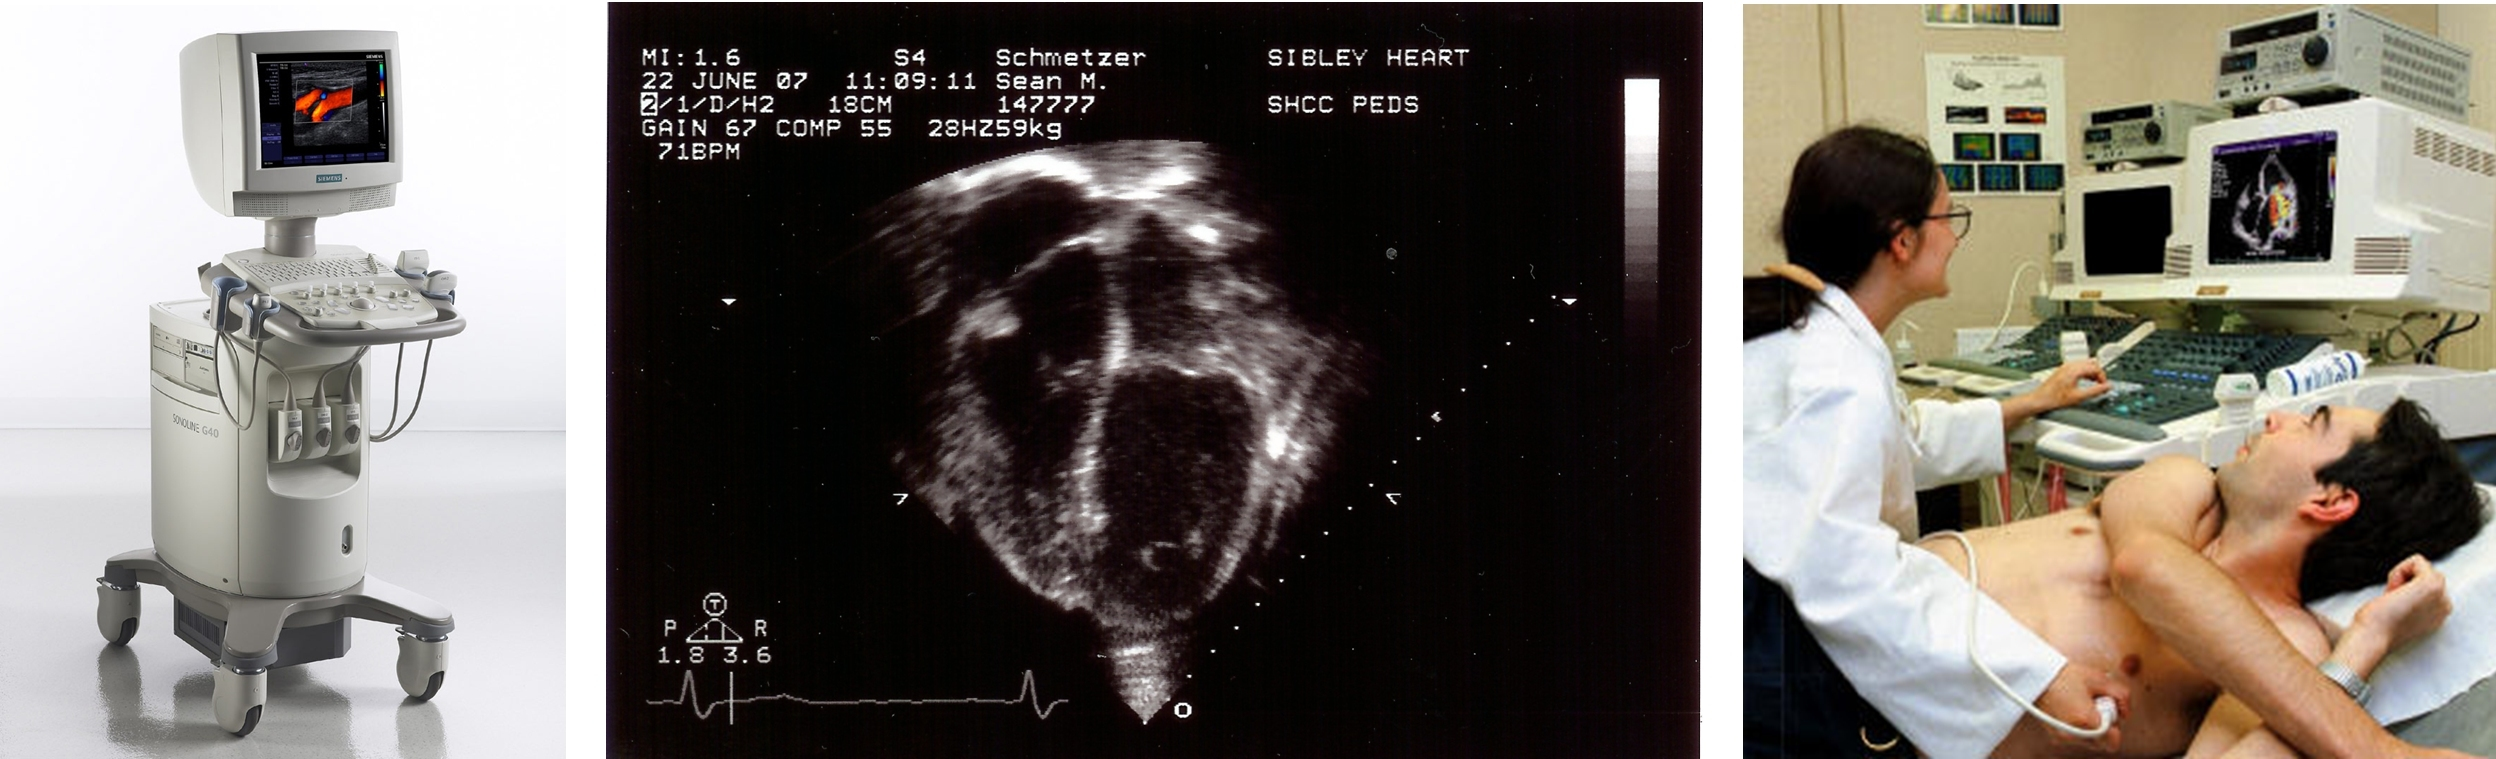
\includegraphics[width=0.6\textwidth]{figures/admittance_control_2_1}
    \caption{Blok-shema admitancijskog upravljanja u kojem se izmjerena kontaktna sila koristi za generiranje korekcija putanje koje izvršava unutarnji pozicijski regulator robota (prilagođeno iz \cite{conti2010interface}).}
    \label{fig:admittance_block}
\end{figure}

\subsection{Usporedna analiza osnovnih upravljačkih pristupa}
Kako bismo olakšali odabir odgovarajuće strategije u dizajnu robotskih ultrazvučnih sustava, u Tablici \ref{tab:usporedba_upravljanja} dan je usporedni prikaz četiriju osnovnih upravljačkih pristupa s njihovim prednostima i ključnim ograničenjima u medicinskom kontekstu.

\begin{table}[H]
\centering
\caption{Usporedba upravljačkih pristupa u robotskom ultrazvučnom snimanju.}
\label{tab:usporedba_upravljanja}
\begin{tabularx}{\textwidth}{p{0.18\textwidth} X X}
\toprule
\textbf{Pristup} & \textbf{Prednosti} & \textbf{Ograničenja / Nedostatci} \\
\midrule
\textbf{Pozicijsko upravljanje} & Jednostavna implementacija, visoka točnost praćenja unaprijed poznatih putanja. & Visok sigurnosni rizik na mekom tkivu, opasnost od prekomjernih sila pri micanju pacijenta, čest gubitak kontakta. \\
\textbf{Izravno upravljanje silom} & Točno održavanje željene sile $F_d$ na zadanoj vrijednosti bez trajnog odstupanja. & Zahtijeva točan dinamički model robota i izravnu kontrolu momenta zglobova; nestabilnost na krutim strukturama (rebra). \\
\textbf{Upravljanje impedancijom} & Visoka sigurnost, prirodno oponaša popustljivost (opruga/prigušivač), izrazito stabilno u interakciji s tkivom. & Zahtijeva napredne robote s kontrolom momenta i mjerenjem struje u zglobovima; teško je ostvariti točno praćenje konstantne sile bez statičke pogreške. \\
\textbf{Upravljanje admitancijom} & Može se primijeniti na krutim industrijskim robotima s pozicijskim sučeljem; visoka stabilnost pri niskim brzinama. & Ovisi o vanjskom F/T senzoru; prisutno je kašnjenje u odzivu zbog unutarnje pozicijske petlje robota. \\
\bottomrule
\end{tabularx}
\end{table}

\subsection{Hibridno upravljanje silom/pozicijom (Hybrid Force/Position Control)}
U robotskom ultrazvučnom snimanju potrebno je istovremeno pomicati sondu duž kože pacijenta (tangencijalno gibanje) i održavati konstantnu silu pritiska u smjeru okomitom na kožu (aksijalno upravljanje) \cite{sciencedirect2025hybrid}. Hibridno upravljanje dijeli prostor zadatka na dva ortogonalna podprostora pomoću selekcijske matrice $S$ i njezine komplementarne matrice $I - S$ \cite{raghavv2022autonomous, ieee2023full}:
\begin{equation{}}
    v_{cmd} = S v_p + (I - S) v_f
\label{eq:hybrid}
\end{equation{}}
gdje su:
\begin{itemize}
    \item $S$ -- dijagonalna selekcijska matrica s elementima $1$ za smjerove u kojima se upravlja pozicijom/brzinom ($v_p$), i $0$ za smjerove u kojima se upravlja silom ($v_f$),
    \item $I$ -- jedinična matrica odgovarajuće dimenzije.
\end{itemize}
Ovaj pristup omogućuje robotičaru da npr. definira smjerove $X$ i $Y$ (paralelne s površinom kože) kao pozicijski kontrolirane, dok se smjer $Z$ (okomit na kožu) kontrolira izravno silom ili admitancijskom petljom \cite{ieee2025cascaded, li2026robotic}.

\subsection{Utjecaj geometrije površine tijela na stabilnost kontakta}
Ljudsko tijelo karakteriziraju izrazito nepravilne i zakrivljene anatomske geometrije (npr. zaobljenost abdomena, zakrivljenost vrata pri snimanju karotidne arterije ili štitnjače). Pri kretanju ultrazvučne sonde duž takvih površina javljaju se značajni problemi za stabilnost kontakta:
\begin{enumerate}
    \item \textbf{Promjena smjera normale:} Sila pritiska mora se uvijek aplicirati okomito na površinu kože (u smjeru lokalne normale) kako bi se osigurao maksimalni prijenos ultrazvučnih valova u tkivo. Kako se sonda pomiče, smjer normale se neprestano mijenja u prostoru \cite{raghavv2022autonomous}.
    \item \textbf{Pojava tangencijalnih sila i momenata:} Ako se orijentacija sonde ne prilagođava zakrivljenosti površine, kontaktna sila više neće djelovati isključivo u aksijalnom smjeru sonde. Javljaju se bočne (tangencijalne) sile koje uzrokuju bočno proklizavanje sonde, naboranje kože pacijenta te narušavanje stabilnosti upravljačke petlje \cite{ieee2023full}.
    \item \textbf{Degradacija ultrazvučnog kontakta:} Kada kut sonde odstupi od normale površine, dolazi do loma i refleksije zvučnih valova pod nepovoljnim kutom, što dovodi do gubitka akustičkog prozora, pojave artefakata i potpunog zatamnjenja ultrazvučne slike \cite{akbari2021robotic}.
\end{enumerate}
Kako bi se ovi problemi riješili, moderni robotski sustavi koriste hibridno upravljanje u kojem se položaj regulira u tangencijalnoj ravnini, sila u aksijalnom smjeru, dok se orijentacija sonde neprekidno prilagođava (automatsko poravnanje) minimiziranjem tangencijalnih momenata izmjerenih na F/T senzoru ($M_x \approx 0, M_y \approx 0$) \cite{conti2010interface} ili na temelju vanjskih 3D kamera koje u realnom vremenu rekonstruiraju geometriju površine pacijenta \cite{ieee2025path}.

